\section{FreeRTOS}
%\note{Kort intro til hvad FreeRTOS er og hvilken funktionalitet det stiller tilrådighed}
Som indlejret styresystem benyttes FreeRTOS. 
FreeRTOS er et open source real-tids styresystem til indlejrede systemer, som er blevet en industriel standard. 
Styresystemet er valgt, da det er simpelt at gå til. 
Det er desuden primært skrevet i programmeringssproget C, som også benyttes i projektet. 
FreeRTOS benytter preemptive schedulering til at administrere CPU-tiden mellem tasks. 

\section{Preemptive schedulering}
FreeRTOS er bygget på en prioritetsbaseret preemptive scheduleringsalgoritme.\newline
Når et operativ system opererer med en preemptive scheduleringsalgoritme kan kørende processer preemptes - blive stoppet - og skiftet ud med en anden proces.\newline
Det kan f.eks. være at en proces der har ventet på en I/O device får tilgang til denne.
Scheduleren vil så skifte den nuværende kørende proces ud og skifte den hidtil ventende proces ind så den kan køres.
Dette gør scheduleren via et context switch.\newline
Når et context switch sker gemmes ''konteksten`` af den nuværende task i en process control block (PCB), og ydermere sker der et state restore, hvor informationen i PCBen af den task, der skal skiftes til hentes.
Det som bliver gemt i PCBen er værdierne i CPU registrene (Program counter, etc.) og anden vigtig operativ systemsinformation.\newline
Prioritetsbaseret skeduleringsalgoritmer tildeler alle tasks en prioritet som er baseret på taskens vigtighed.\newline
FreeRTOS er et real-time operativ system og et primært formål ved real-time operativ systemer er at give et respons på begivenheder indenfor en vis deadline.
FreeRTOS skeduleringsalgoritme sørger så for at den task med højest prioritet bliver givet processortid.

\section{Løsningsimplementering og task model}
\begin{figure}[h]
	\centering
	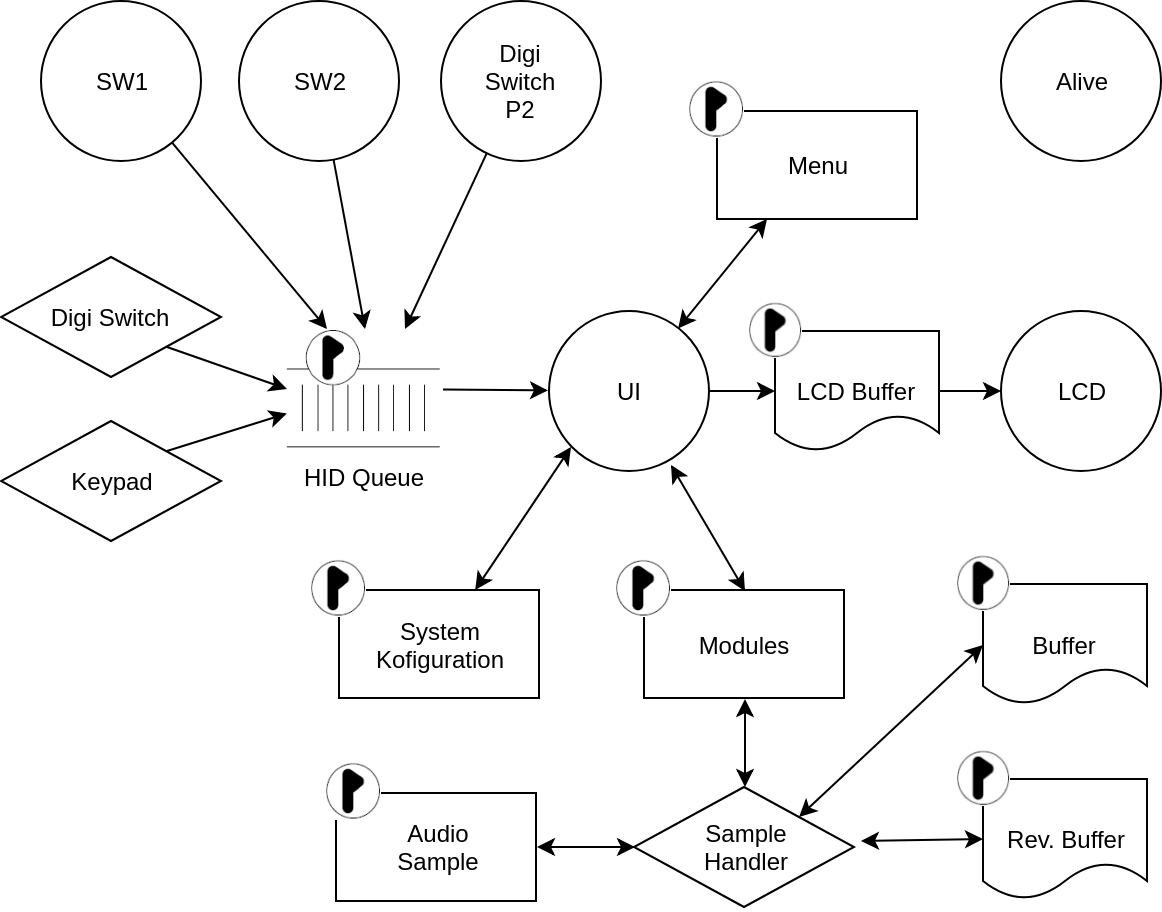
\includegraphics[width=.9\linewidth]{billeder/taskmodel.png}
	\caption{Task model af den implementrede løsning.}
	\label{fig:taskmodel}
\end{figure}
Figur \ref{fig:taskmodel} vise en oversigt over de task der køre i løsningen.
Som udgangspunkt ligger \texttt{UI} tasken som den centrale del der styre konfigurationen, menusystemet.
Alt input fra HID\footnote{HID - Human Inputer Devices} enhederne på emp-printes - tastatur, switches og digiswitch, bliver sendt ind i en kø med en fast defineret datastruktur som se i figur \ref{fig:hid_msg_t}, og som \texttt{UI} tasken således er forbruger af.
\lstset{language=C,
	frame=sigle,
	basicstyle=\ttfamily\tiny,
	emph={uint8_t,hid_msg_t},
	emphstyle={\color{blue}},
	keepspaces=true,
	frame=single,
	%	numbers=left,
	%	numbersep=5pt,
	numberstyle=\tiny\color{black},
	keywordstyle=\color{red}\ttfamily,
	stringstyle=\color{blue}\ttfamily,
	commentstyle=\color{OliveGreen}\ttfamily,
	morecomment=[l][\color{magenta}]{\#}
}
\begin{figure}[h!]
\begin{tabular}{l}
	\begin{lstlisting}
		typedef struct hid_msg {
		uint8_t   ch;             // ASCII char kode
		uint8_t   function;       // Funktionskode defineret af HID_FUNC_xxx
		uint8_t   event;          // Eventkode definederet af HID_EVENT_xxx
		} hid_msg_t;
	\end{lstlisting}
\end{tabular}
\caption{struct hid\_msg\_t}
\label{fig:hid_msg_t}
\end{figure}

Datastrukturen \texttt{Menu} indeholder den dynamiske pointer struktur til menusystemet der bliver beskrevet i afsnit \ref{sec:HID} på side \pageref{sec:HID} og datastrukturerne \texttt{System konfiguration} og \texttt{Modules} indeholder information til styring af systemet som helhed, herunder mono/stereo mode og hvilke enheder der er anvendes som audio ind/ud.

LCD diaplayet bliver hold opdateret af en \texttt{LCD} task, der løbende overfører tegn fra \texttt{LCD bufferen}, dette system er nærmere beskrevet i afsnit \ref{sec:LCD_driver}.

Den grundliggende timing og lydbehandling styres igennem \texttt{Sample Handler} ISR\footnote{ISR - Interrupt Service Routine}.
Denne ISR sørger for at hente lyddata fra ADC'en, finder frem til hvilke moduler der skal medtages i databehandlingen og hvordan og til hvilke buffere, \texttt{Buffer} eller \texttt{Rev. Buffer} data skal gemmes i.
Der vil i de efterfølgende afsnit komme en mere uddybende gennemgang for hver af systemets tasks og implementeringer. 


\section{Intterrupt eksekvering og task skedulering}
\label{subsec:int_task}
Figur \ref{fig:int_task} viser hvordan tasks og interrupts håndteres i FreeRTOS. 
Til tiden t1 kører en lavt prioriteret task. 
Ved t2 bliver en interrupt service rutine, fremover kaldet en ISR, kaldt. 
Den prioriteres højest, og den lavt prioriteret task pauses indtil ISR'en er færdig.
ISR'eren er færdig til tiden t3, hvor den lavt prioriteret task kan genoptages.
Ved t4 sker et context switch til en højere prioriteret task.
Skeduleringen mellem tasks er styret af FreeRTOS scheduler med respekt til den prioritet, som hver task er givet. 
Interrupts prioriteres højere end alle tasks, uanset prioriteten af den pågældende task. 
Interrupts har også prioriteter i mellem sig, såfremt flere skulle blive kaldt. 
Modsat tasks, vil en interrupt dog altid afsluttes, før den næste kan begynde. 
ARM Cortex-M4 tilbyder otte interrupt prioriteter. 
\husk{Jes}{Forstået rigtigt?} 
\begin{figure}[h]
	\caption{Det tidslige forløb for to tasks og en interrupt service rutine. }
	\centering
	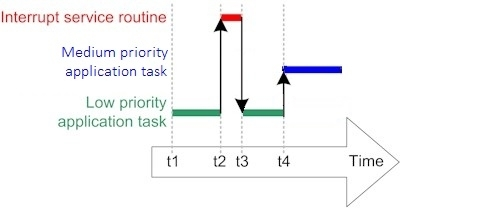
\includegraphics[width=0.6\linewidth]{billeder/interruptandtaskprocessing.jpg}
	\label{fig:int_task}
\end{figure}

Når det indgående lydsignal skal samples gennem ADC'en, skal samplingen foregå periodisk på nøjagtigt det samme tidspunkt i hver periode.
Det faste tidspunkt for sampling giver minimal jitter med en minimal forsinkelse i samplingen af signalet. 
%\husk{Jes}{Dansk ord for jitter? Det er et teknisk engelsk ord, så det kan vel gå.. } 
For at sikre, at mikrocontrolleren sætter alle andre opgaver på pause, og begynder at sample på det korrekte tidspunkt, implementeres samplingen i en ISR.

\subsection{Implementering af interrupt-styring med timer}
\label{subsec:impl_int}
ISR'en indstilles med den højest mulige interrupt prioritet. 
Timingen af ISR'en er styret af Timer 3. 
Timeren er implementeret som en 16-bit timer i periodic timer mode, edge-count mode og inverted PWM mode.
Ved start hentes timerens start value ind i et tælleregister. 
Sample-frekvensen og CPU frekvensen styrer værdien. 
\begin{equation}
	\text{Timer start value register} = \frac{\text{CPU'ens frekvens}}{\text{Sample-frekvens}} = \frac{80\text{MHz}}{44,1\text{kHz}} \simeq 1814
\end{equation}
I periodic timer mode vil timeren dekrementere fra tælleregisteret, som automatisk henter timer start værdien igen, og begynder forfra når værdien når nul. 
Når værdien når nul, kaldes den ISR som sikrer at lydsignalet bliver samplet. \newline

\section{Sampling af lydsignal igennem ADC}\label{sec:ADC}
Microcontrolleren har to identiske ADC moduler, som opererer uafhængigt ad hinanden. 
De kan derfor sample på samme tidspunkt. 
ADC'erne er opbygget med Successive Approximation Register arkitektur, som leverer en opløsning på 12-bit, hvilket giver 4096 mulige steps i det digitale resultat. 
ADC'ens interne forsyningsspænding og ground er på henholdsvis 3,3V og 0V, hvilket samtidig er den maksimale og minimale spændingsreference, som ADC'en kan læse. 
Stepsizen er $\Delta$ er udregnet i formel \ref{eq:ADC_res}.
\begin{equation}
\label{eq:ADC_res}
	\Delta = \frac{X_{maks}-X_{min}}{steps} = \frac{3\text{V}-0\text{V}}{4096} = 0,73\text{mV}
\end{equation}
\husk{Jes}{Stepsize udregning kan måske udelades, hvis vi får pladsmangel.}
ADC'en er drevet af en 16MHz clock, og det tager 250ns at tage én sample. 

\subsection{Opsætning af ADC}
ADC0 og ADC1 er sat op til at modtage et analogt signal, for henholdsvis venstre og højre kanal, direkte på to general purpose input pins (GPIO). 
Start af sampling er indstillet, så det trigges af et processor event. 
Det betyder at en sampling i praksis startes ved at skrive til ADC Processor Sample Sequence Initiate registeret. 
Resultatet af en A/D konvertering kan læses i sequence 3. 
ADC'en har fire individuelle sequence registre, som kan indeholde op til flere samples efter FIFO princippet. 
Sequence 3 er valgt, da den kun kan indeholde én sample, hvilket er praktisk når samplingens timing skal være præcis. 
Yderligere samples ville ikke være brugbare, fordi de ville være målt på et forkert tidspunkt. 

\subsection{ISR sample handler og ADC}
Som nævnt i afsnit \ref{subsec:int_task}, vil det timerstyrede interrupt kalde sample handler rutinen.
I rutinen startes samplingen som det allersidste. 
Det betyder at dataene fra samplingen bliver gemt i sequence 3 registeret indtil næste gang interruptet kaldes. 
Næste gang interruptet kaldes, gemmes dataene i en variabel, og en ny AD konvertering bliver herefter igen udført. 
Fordelen er at hver gang ISR'en bliver kaldt, vil samplen ligge klar.
Der skal ikke ventes på en konvertering. 
Det betyder også at forsinkelsen fra en konvertering bliver konstant. Forsinkelsen vil være givet ved $\frac{1}{f_s}$. 

\subsection{Offset af samplet data}
Værdien af den modtagede sample fra AD konverteringen vil have et offset pga. DC forskydningen ved input stage, som tidligere beskrevet i afsnit \ref{sec:inputstage}.
Offsettet fjernes igen ved at trække $\frac{4096}{2} = 2048$ fra resultatet af AD konverteringen. 
Resultatet gemmes som en værdi af data typen float. 
\husk{Jes}{Hvis der er plads, kunne det være rart med en graf her.}

\subsection{Sample handler og processortid}
Da sample handleren kører periodisk, og i form af en ISR har højeste prioritet til processortid, skal alle andre processoropgaver foregå i al den mellemliggende tid. 
Det betyder at sample handleren og AD konverteringen skal være tidseffektiv, således andre tasks kan nå at køre færdig, inden sample handleren kaldes igen. 
Ved hjælp af timer 3, udregnes rutinens procentuelle andel af processortiden, hvilket kan skrives ud til brugeren ved brug af LCD displayet. 
Den benyttede tid vil desuden være afhængig af antallet af modulære effekter, som også skal processeres i sample handleren. 

\section{Modulær opbygning af effekter}
Effektmodulerne holdes hver især i en \textit{module control block}, $\mathtt{mcb\_t}$,  som er en data struktur bestående af en \textit{function pointer} og en booleansk variabel.
Function pointeren benyttes til at kalde lydeffektmodulerne, og den booleanske variabel benyttes til at aktivere/deaktivere lydeffekterne.\newline
For at tilføje en lydeffekt laves der en ny instans af $\mathtt{mcb\_t}$, og dens \textit{function pointer} sættes til at \textit{pointe} til lydeffekt rutinen.\newline
\begin{figure}[!ht]
	\centering
	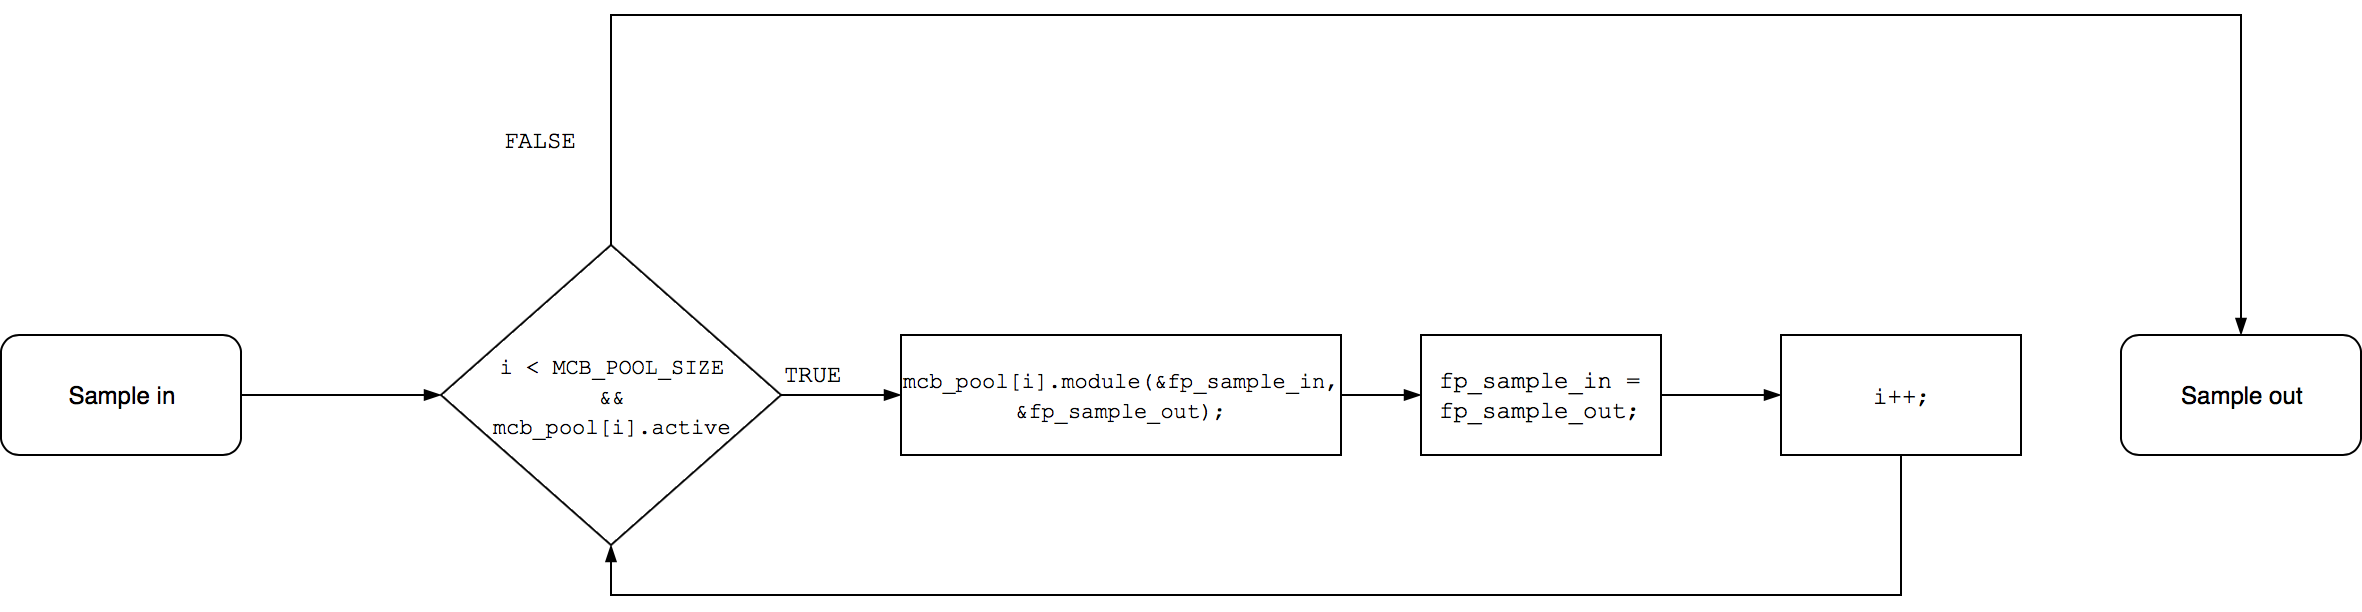
\includegraphics[width=\textwidth]{billeder/Flowchart_for_effektmoduler.png}
	\caption{Flowchart for iteration gennem effektmoduler}
	\label{fig:effektmoduler}
\end{figure}

På figur (\ref{fig:effektmoduler}) illustreres det, hvordan de enkelte moduler bliver itereret over, hvis de er aktive.
Hvori $\mathtt{MCB\_POOL\_SIZE}$ er antal af moduler, $\mathtt{mcb\_pool}$ er en array af $\mathtt{mcb\_t}$ strukturer, $\mathtt{mcb\_pool.module}$ er \textit{function pointeren}, $mathtt{mcb\_pool.active}$ er den \textit{booleanske} variabel og $\mathtt{fp\_sample\_in}$ og $\mathtt{fp\_sample\_out}$ er hhv. input- og outputsamples.
Grunden til at outputtet fra hver modul bliver sat til input, er at det ønskes at opnå en seriel kobling af effekterne.
For at tilføje et effektmodul oprettes tilføjes der et nyt element til $\mathtt{mcb\_pool}$, \textit{function pointerent} sættes til at \textit{pointe} til effektroutinen og den booleanske variabel sættes til $\mathtt{TRUE}$.

\section{Generering af PWM-signal til DAC}
Timeren benyttes desuden til at generere et PWM-signal, hvis duty cycle er styret af timeren og resultatet af A/D konverteringen af indgangssignalet. 
\begin{wrapfigure}[15]{r}{0.5\textwidth}
	\centering
	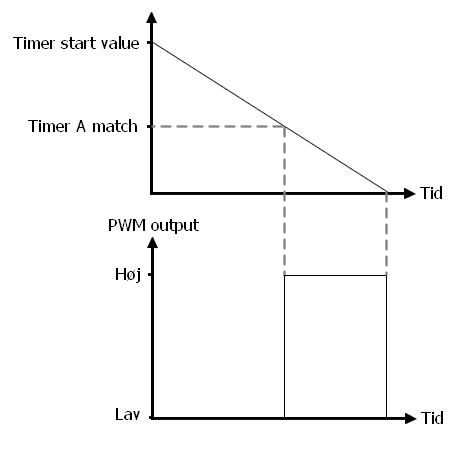
\includegraphics[width=0.5\textwidth]{billeder/timer3PWM.png}
	\caption{\label{fig:PWMfromtimer}Generering af PWM-signal ud fra timer. }
\end{wrapfigure}
Figur \ref{fig:PWMfromtimer} viser hvordan PWM-signalets duty cycle bliver bestemt af den værdi, som bliver gemt på Timer A's match register. 
Den værdi kommer fra den periodiske sampling af lydsignalet gennem ADC'en, hvor resultatet af hver sampling netop gemmes i match registeret. 
Således genskabes signalet som et digitalt PWM signal. 

\section{Genskabelse af signal via DAC igennem SPI}
Genskabelsen af udgangssignalet fra mikorcontrolleren gøren igennem en ekstern 12bit DAC \texttt{MCP4922E/P}\footnote{Microchip MCP4922E/P 12-Bit Dual Voltage Output Digital-to-Analog Converter with SPI Interface \cite{mcp4922} }.



\section{LCD Driver}
\label{sec:LCD_driver}
Når $\mathtt{lcd\_write\_char}$, $\mathtt{lcd\_write}$ og $\mathtt{lcd\_clear}$ bliver kaldt bliver deres argumenter sat over i en LCD buffer, $\mathtt{lcd\_display\_buffer}$.
Når de så skal skrives til LCDen tager LCD tasken sig af at skrive til skærmen, når scheduleren når til tasken.
\begin{figure}[!ht]
	\centering
	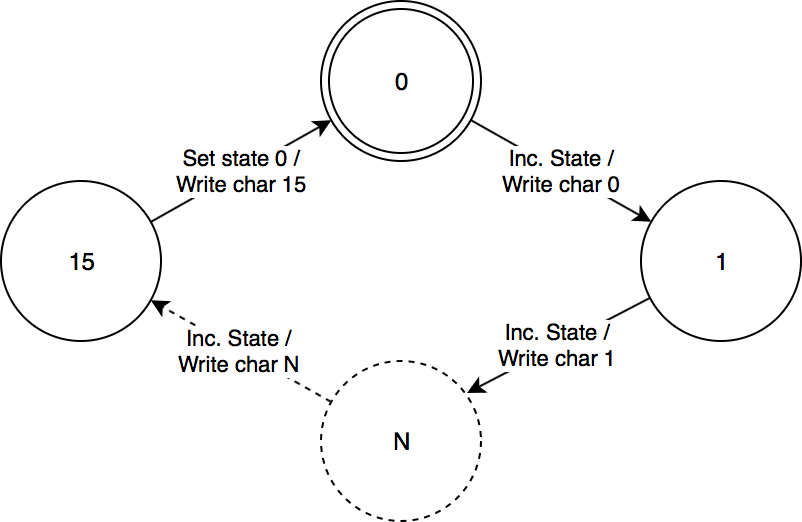
\includegraphics[width=0.5\textwidth]{billeder/lcd_state_machine.png}
	\caption{LCD state machine}
	\label{fig:LCD_state_machine}
\end{figure}
\newline
Måden LCD tasken virker på er, at den har en state machine som er vist på figur (\ref{fig:LCD_state_machine}).\newline
I state machinen bliver der itereret gennem $\mathtt{lcd\_display\_buffer}$, hvori der kaldes $\mathtt{lcd\_direct\_write\_data\_nodelay}$ på bufferen med $\mathtt{state}$ som index.\newline
$\mathtt{lcd\_direct\_write\_data\_nodelay}$ som er en skrivefunktion som ikke har noget \textit{end delay}.
Når $\mathtt{state}$ når $16$ skrives der videre på næste linje.

\section{Håndtering af brugergrænseflade og human input interface}
\label{sec:HID}
%For at kunne anvende enheden skal enheden kunne udveksle nødvendige informationer med brugeren, input skal altså kunne modtages, her valgte gruppen at anvende en "drehimpulsgeber", og respons skal oplyses, her valgte gruppen et grafisk repræsenteret menu system.
For at kunne anvende enheden skal enheden kunne udveksle nødvendige informationer med brugeren. 
Input skal kunne modtages, her valgte gruppen at anvende en "drehimpulsgeber" eller digiswitch, samt to switches.
Respons skal oplyses, her valgte gruppen et grafisk repræsenteret menu system.
%En menu består en række valgmuligheder repræsenteret af elementer brugeren kan bladre igennem og vælge imellem.
En menu består af en række valgmuligheder repræsenteret af elementer brugeren kan bladre igennem og vælge imellem.
Et valg kan lede til yderligere valgmuligheder inden for den valgte kategori, disse kan så præsenteres i form af en ny menu.
\begin{figure}[!ht]
	\centering 
	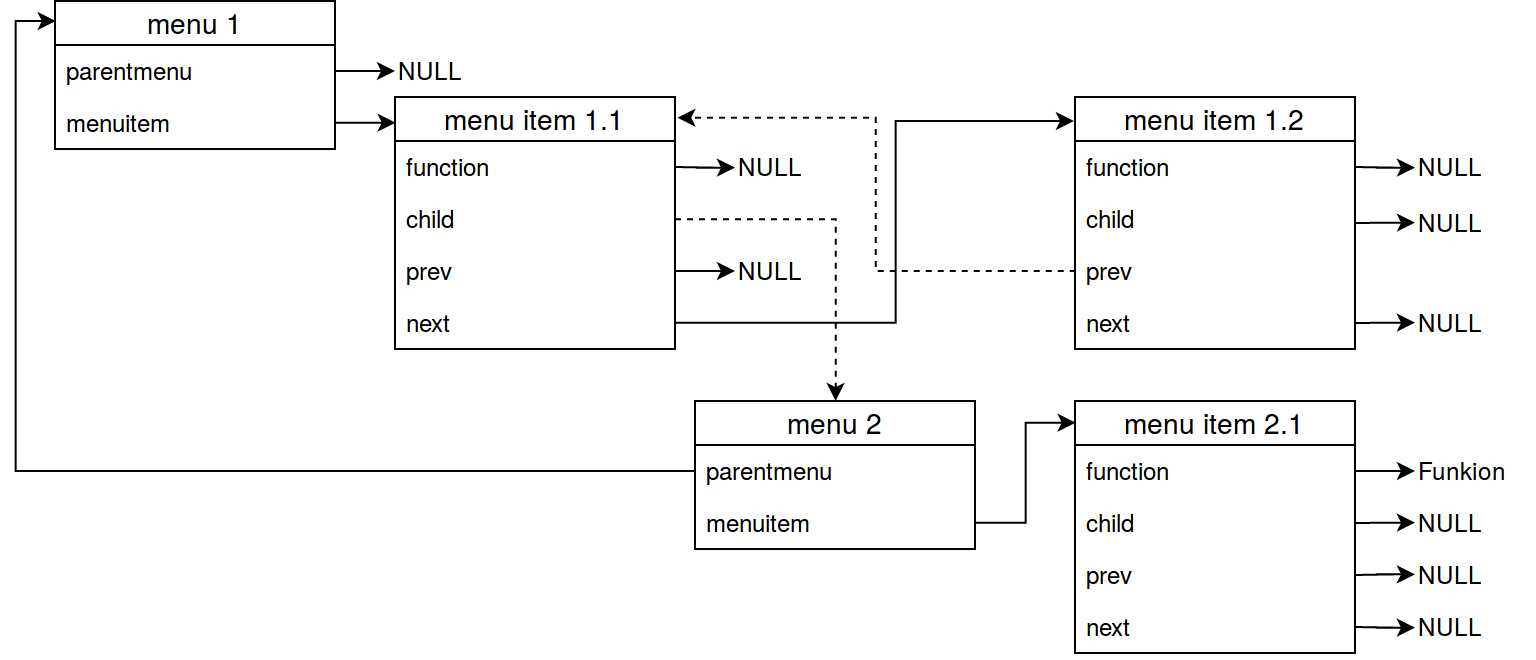
\includegraphics[width=0.8\textwidth]{billeder/menuesdiagram.png} 
	\caption{Generisk diagram over menu datastruktur. } 
	\label{fig:menuesdiagram} 
\end{figure}
Til at udføre denne funktion valgte gruppen at anvende linkede lister.\newline
%I eksemplet herunder ses en hovedmenu "Root Menu" som linker til sit første element "Master volume", vælger brugeren dette element kan volumen sættes, elementet linker også til næste element så brugeren kan skifte til det, her er der tale om "Echo" elementet som istedet for at have en funktion linker til en ny menu nemlig "Echo menu" som så linker til sin egen liste af menu punkter.
På figur \ref{fig:menuesdiagram} ses en hovedmenu ''menu 1`` som linker til sit første element ''menu item 1.1``, herfra kan brugeren bladre til næste element ''menu item 1.2`` eller vælge dette element, vælges elementet ''menu item 1.1`` ses det på diagrammet at under menuen ''menu 2`` åbnes, derved vises nu første element fra ''menu 2`` som er ''menu item 2.1`` som har en funktion brugeren kan anvende.
%kan volumen sættes.
%Elementet linker også til næste element så brugeren kan skifte til det, her er der tale om ''Echo`` elementet som i stedet for at have en funktion linker til en ny menu nemlig ''Echo menu`` som så linker til sin egen liste af menu punkter.
%En "drehimpulsgeber" kan anvendes til at producere 3 forskellige typer af input, drej mod uret herefter kaldet "vr", drej med uret "hr" og click.
%Når et input  modtages af programmet lægges det i en input kø til systemet er klar til at modtage input, er der tale om et "vr" fremvises foregående element i menuen, på samme måde anvendes et "hr" input til at gå til næste element i menuen og et click anvendes til at vælge det det nuværende element.
Drehimpulsgeberen kan anvendes til at producere 4 forskellige typer af input, drej mod uret herefter kaldet ''Dl``, drej med uret ''Dr``, click og langt tryk.


\begin{wrapfigure}[14]{r}{0.5\textwidth} 
	\centering 
	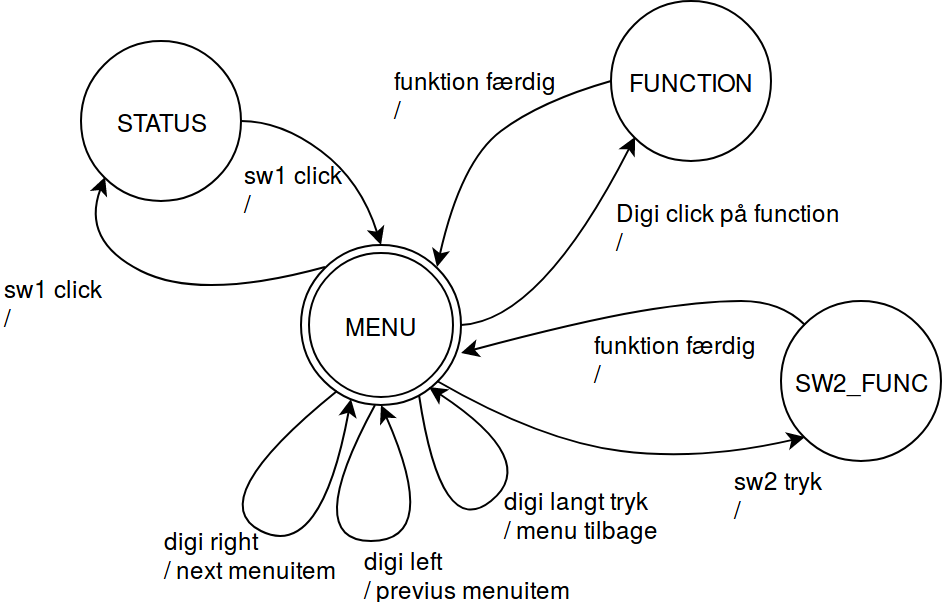
\includegraphics[width= 0.5\textwidth]{billeder/ui_statemachine.png} 
	\caption{UI state machine diagram. } 
	\label{fig:uistatemachine} 
\end{wrapfigure}

Når et input  modtages af programmet lægges det i en input kø til systemet er klar til at modtage input. Er der tale om et ''Dl`` fremvises foregående element i menuen, på samme måde anvendes et ''Dr`` input til at gå til næste element i menuen, et click anvendes til at vælge det nuværende element og et langt tryk til at gå tilbage fra undermenuer.

På figur \ref{fig:uistatemachine} ses den state machine der styre UI.
UI'en der skrives til displayet afhænger af hvilken state der er aktiv.

I staten MENU vises det overordnede menu system, styret af drehimpulsgeberen. 
Er STATUS staten aktiv vises en skærm hvor CPU loaden kan læses.
FUNCTION staten aktiveres hvis der vælges en funktion i menusystemet, i denne state bliver en funktion kaldt fra et af effektmodulerne, denne funktion skriver selv input, og  UI til displayet.
Når denne funktion ikke længere skal bruges, hvis brugeren for eksempel går tilbage, vil state machinen skifte tilbage til MENU.
SW2$\_$FUNC fungere på samme måde. \newline
Tryk på de to switches og den integrerede switch i drehimpulsgeberen håndteres af tre identiske state machines, et diagram over statemachinen ses på figur \ref{fig:SW_statemachine}.

Rotation af drehimpulsgeberen generere impulser på to forskellige pins henholsvis A og B.
Afhængig af rotationsretningen skifter de ene før den anden. 
Et interrupt er sat til at trigger på både stigende og faldende flanker af pin A.
Interrupthandleren Følger algoritmen der ses på figur \ref{fig:digiFlow}.\newline
\begin{figure}[!ht]
	\centering
	\begin{minipage}[b]{0.50\textwidth}
		\centering 
		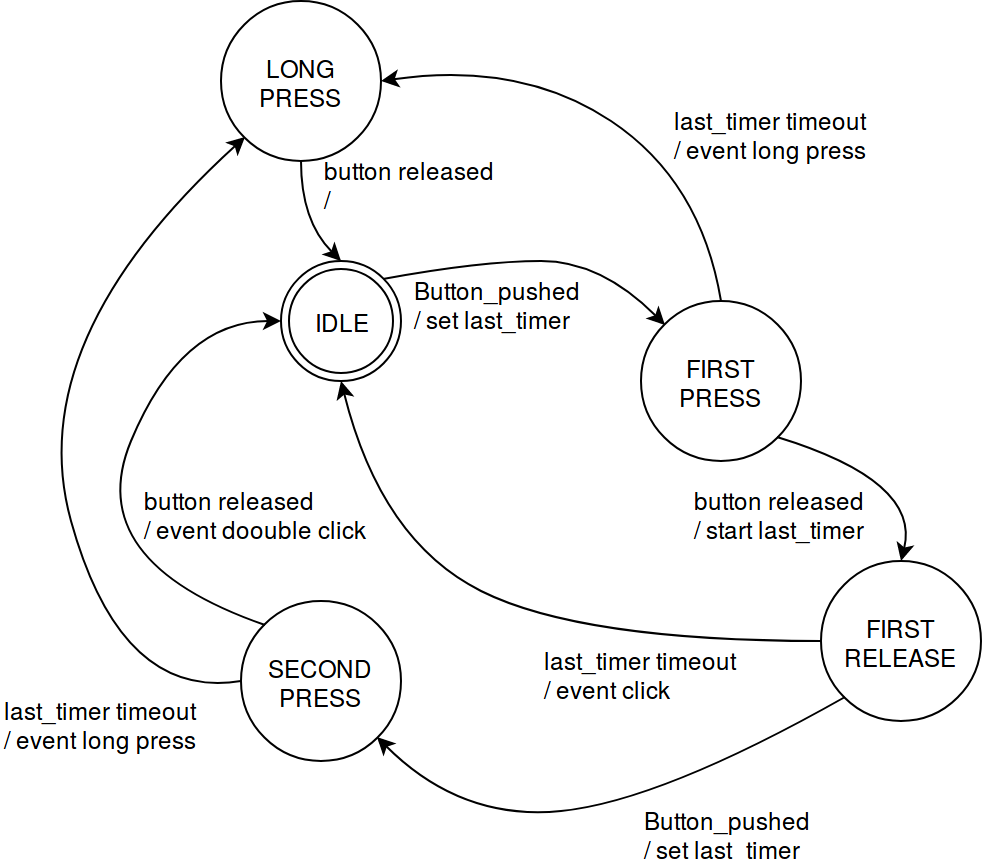
\includegraphics[width=0.8\textwidth]{billeder/buttons_statemachine.png}
		\newline 
		\caption{State machine diagram for switches. } 
		\label{fig:SW_statemachine}
	\end{minipage}\hfill
	\begin{minipage}[b]{0.50\textwidth}
		\centering 
		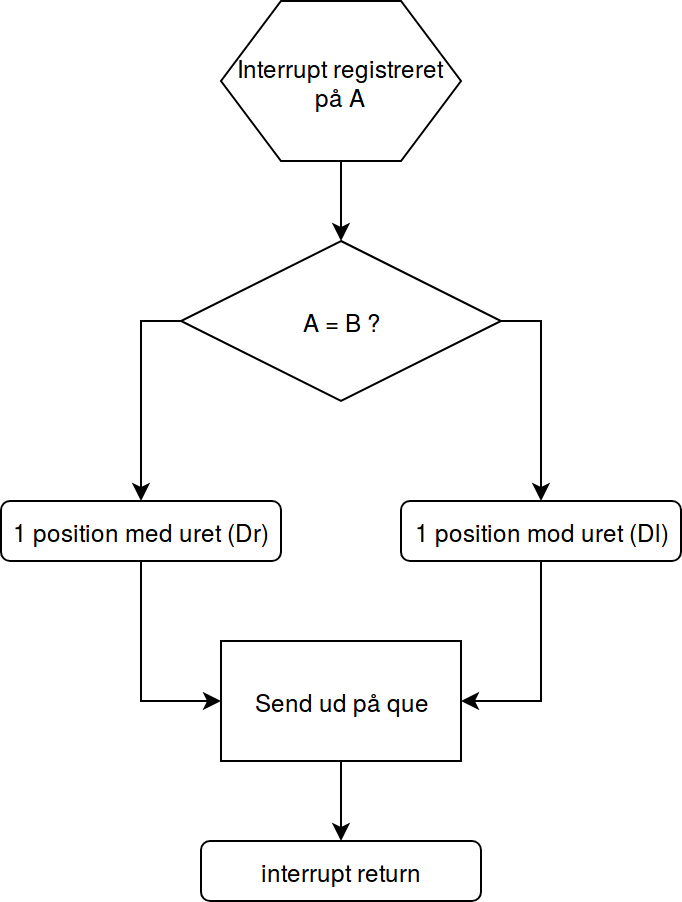
\includegraphics[width=0.8\textwidth]{billeder/digi_interrupt_flow.png} 
		\caption{Flowchart af interrupthandleren til drehimpulsgeberen. } 
		\label{fig:digiFlow} 
	\end{minipage}
\end{figure}
\pagebreak
\section{Opsummering}
FreeRTOS' scheduleringsalgoritme er en prioritetsbaseret preemptive scheduler.
Dette vil sige at hver task bliver givet en prioritet, og hvis en task med en højere prioritet kommer i ready queuen bliver den nuværende task \textit{preemptet}.


De enkelte effektmoduler holdes i en datastruktur indeholdende en \textit{function pointer} og en booleansk variabel.
For hver gang der bliver samplet bliver der itereret over en array af effektmodul data strukturen, og de indeholdende routiner bliver kaldet i samplehandleren som set på figur (\ref{fig:effektmoduler}).\newline
Det eneste der skal gøres for at tilføje et nyt modul er at tilføje et element til arrayen af effektmoduler, sætte \textit{function pointeren} til at pege på effektroutinen og sætte den booleanske variable til true.
Outputtet af hver effekt bruges som input til den næste således at der opnås en kaskadekobling.\newline

LCD-driveren virker ved at write funktioner smider deres resultater over i en buffer.
Når LCD-tasken kører bliver der itereret gennem bufferen, og indholdet af bufferen bliver skrevet ud på LCDen som vist via. figur (\ref{fig:LCD_state_machine}).